\subsection{Hibernate}
\begin{frame}{Implémentation}{Hibernate}
	\begin{minipage}{0.4\textwidth}
		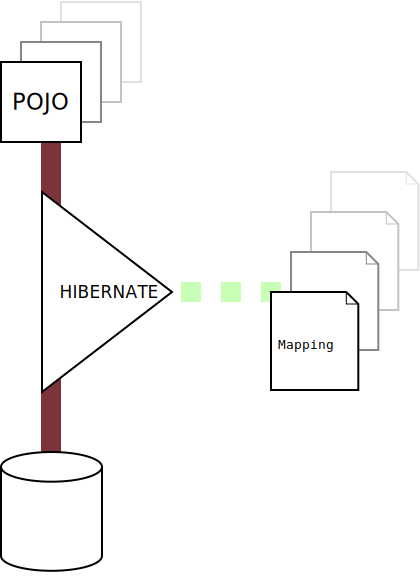
\includegraphics[width=0.8\textwidth]{files/hibernate}	
	\end{minipage}
	\begin{minipage}{0.55\textwidth}
		\begin{itemize}
		\item Framwork ORM Java
		\item Objets POJO
		\item Mapping
		\end{itemize}
	\end{minipage}
\end{frame}

\subsection{Structure de l'application}
\begin{frame}{Implémentation}{Structure de l'application}
	\begin{minipage}{0.4\textwidth}
		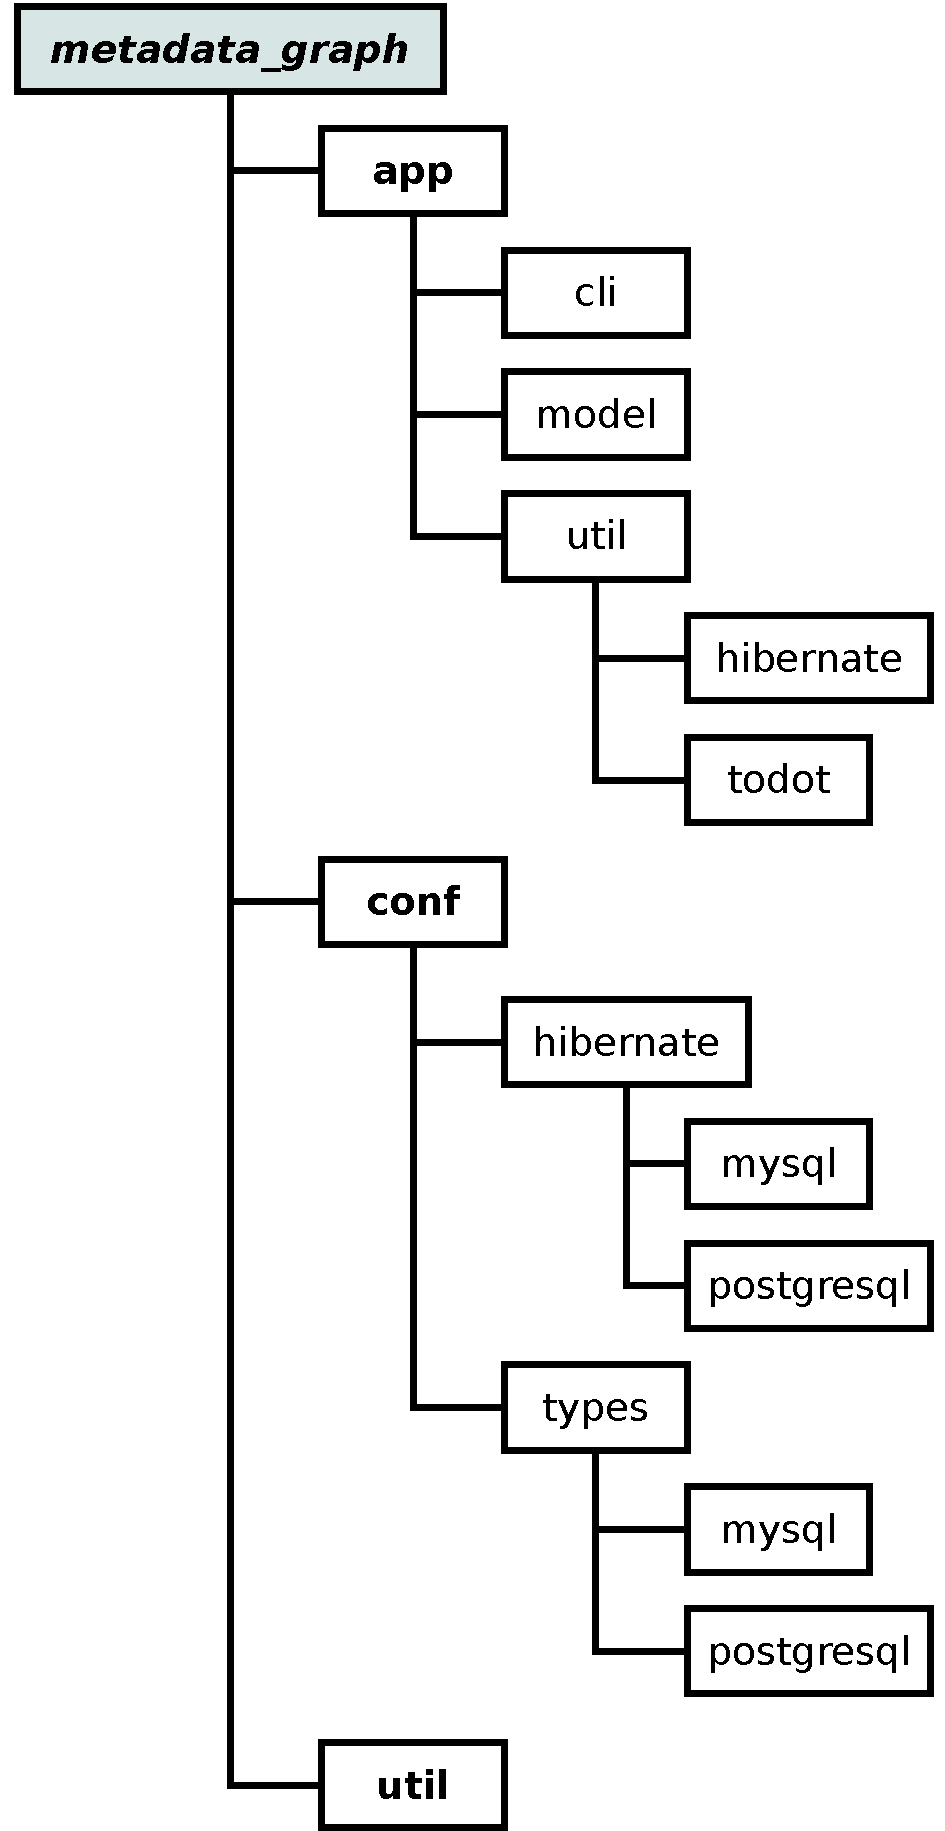
\includegraphics[width=0.8\textwidth]{files/archi}	
	\end{minipage}
	\begin{minipage}{0.55\textwidth}
		\begin{itemize}
		\item Paquet applicatif
		\item Paquet de configuration
		\item Paquet utilitaire
		\end{itemize}
	\end{minipage}
\end{frame}

\subsection{Paquets}
\begin{frame}{Implémentation}{Paquets}
	\begin{block}{\texttt{app.cli}}
	Gestion de l'interface en ligne de commande.
	\end{block}
	\begin{block}{\texttt{app.model}}
	Définition des classes POJO enrichies :
	\begin{itemize}
	\item \texttt{isPK()}
	\item \texttt{isFK()}
	\item \texttt{isCheck()}
	\item \texttt{getGenericType()}
	\end{itemize}
	Énumération des types génériques
	\end{block}
\end{frame}

\begin{frame}{Implémentation}{Paquets}
	\begin{block}{\texttt{app.util}}
	\begin{itemize}
		\item \underline{ToDotUtil} : génération de code au format DOT
		\item \underline{Hibernate} : construction de sessions Hibernate
		\item \underline{Type générique} : fournit le type générique en fonction du SGBD et du type réel
	\end{itemize}
	\end{block}
	
	\begin{block}{\texttt{conf.hibernate}}
	Stocke les fichiers de mapping.
	\begin{itemize}
		\item Le subselect
		\item Problématique de la relation \textit{Many-to-Many}
	\end{itemize}
	\end{block}
\end{frame}

\begin{frame}{Implémentation}{Paquets}
\begin{center}
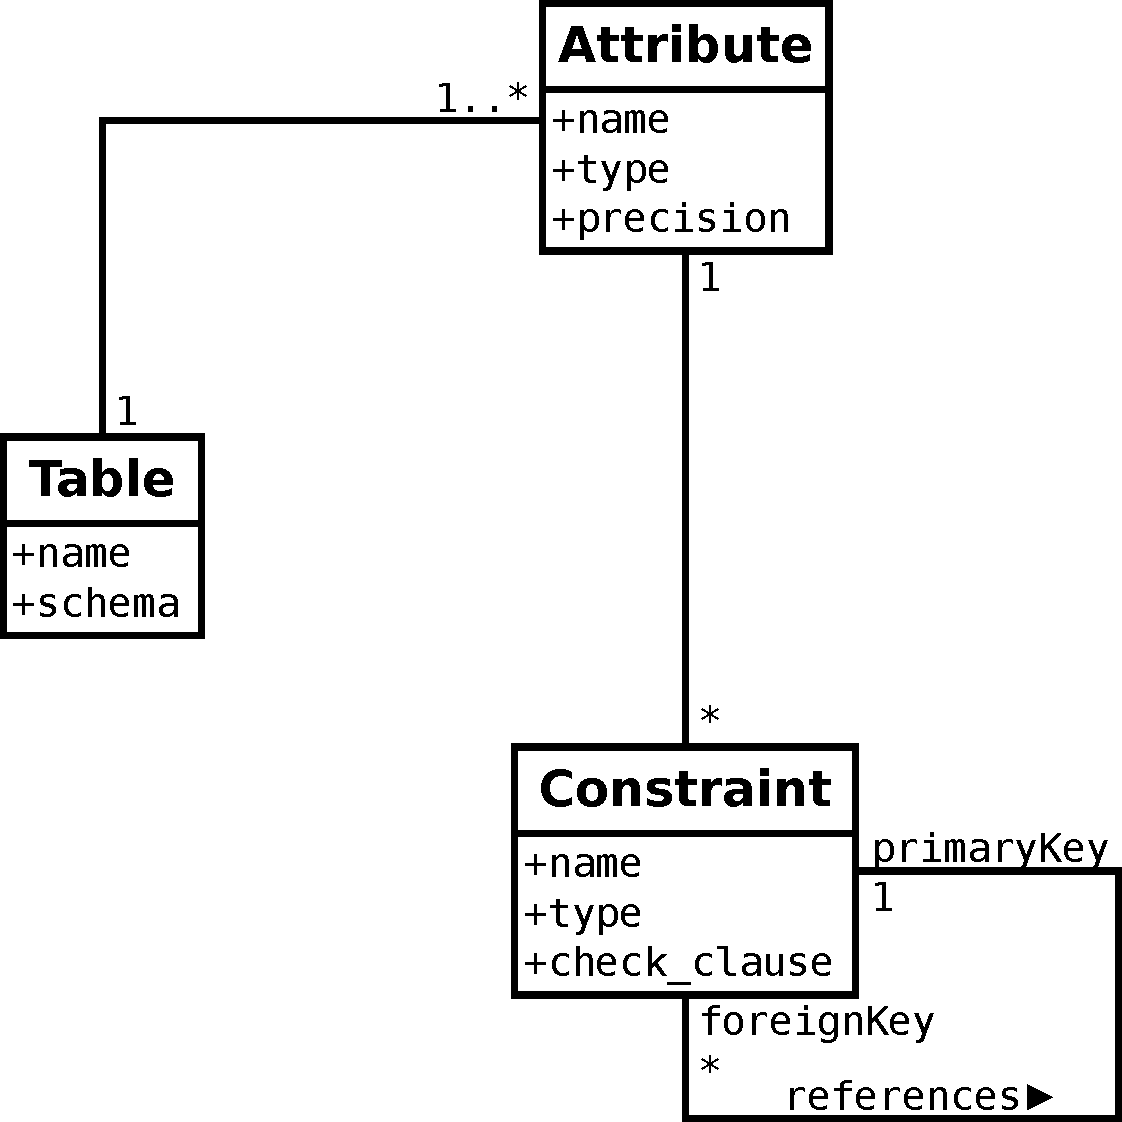
\includegraphics[width=0.5\textwidth]{files/diag_class_final}
\end{center}
\end{frame}

\begin{frame}{Implémentation}{Paquets}
	\begin{block}{\texttt{conf.types}}
	Définition de correspondances (fichiers xml)
	\begin{center}
		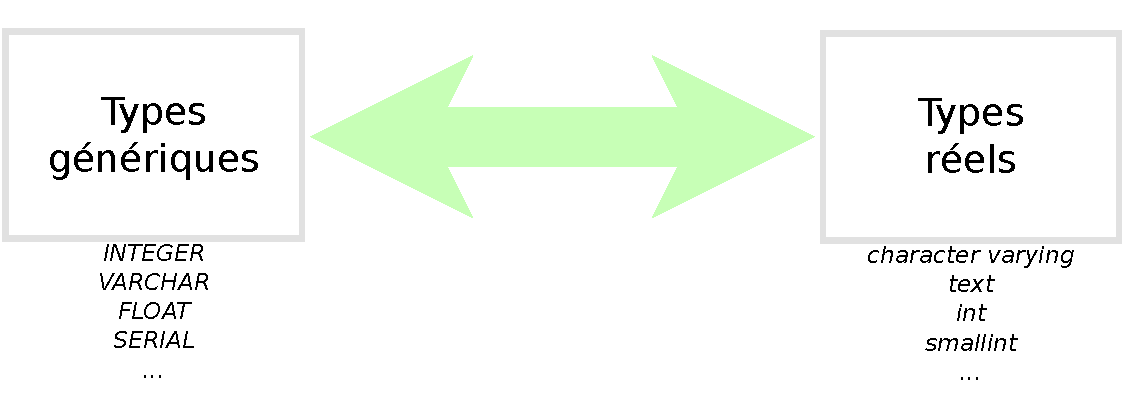
\includegraphics[width=0.8\textwidth]{files/generic_types}	
	\end{center}
	\end{block}
\end{frame}